% Chapter 7

\begin{savequote}[45mm]
Modified\ldots
\qauthor{Ancient proverb}
\end{savequote}

\chapter{Application: Modified SFC} % Main chapter title

\label{Chapter7} % For referencing this chapter elsewhere, use \ref{Chapter7}

%----------------------------------------------------------------------------------------
%	SECTION 1
%----------------------------------------------------------------------------------------

\section{Introduction}

Modifiers in SFC are incompatible with FID, but if you add a fast CG as a
detector, then the volatile modifier is separated from the analytes, and the
modifier elutes as a solvent front, leaving the GC peaks uninterfered with.


\section{(Modified SFC)×GC}

\subsection{Sample}

\subsection{SFC}

\subsection{Modulation}

\subsection{GC}

\subsection{Results}

See Figure \ref{fig:Modifier}

\begin{figure}
	\centering
	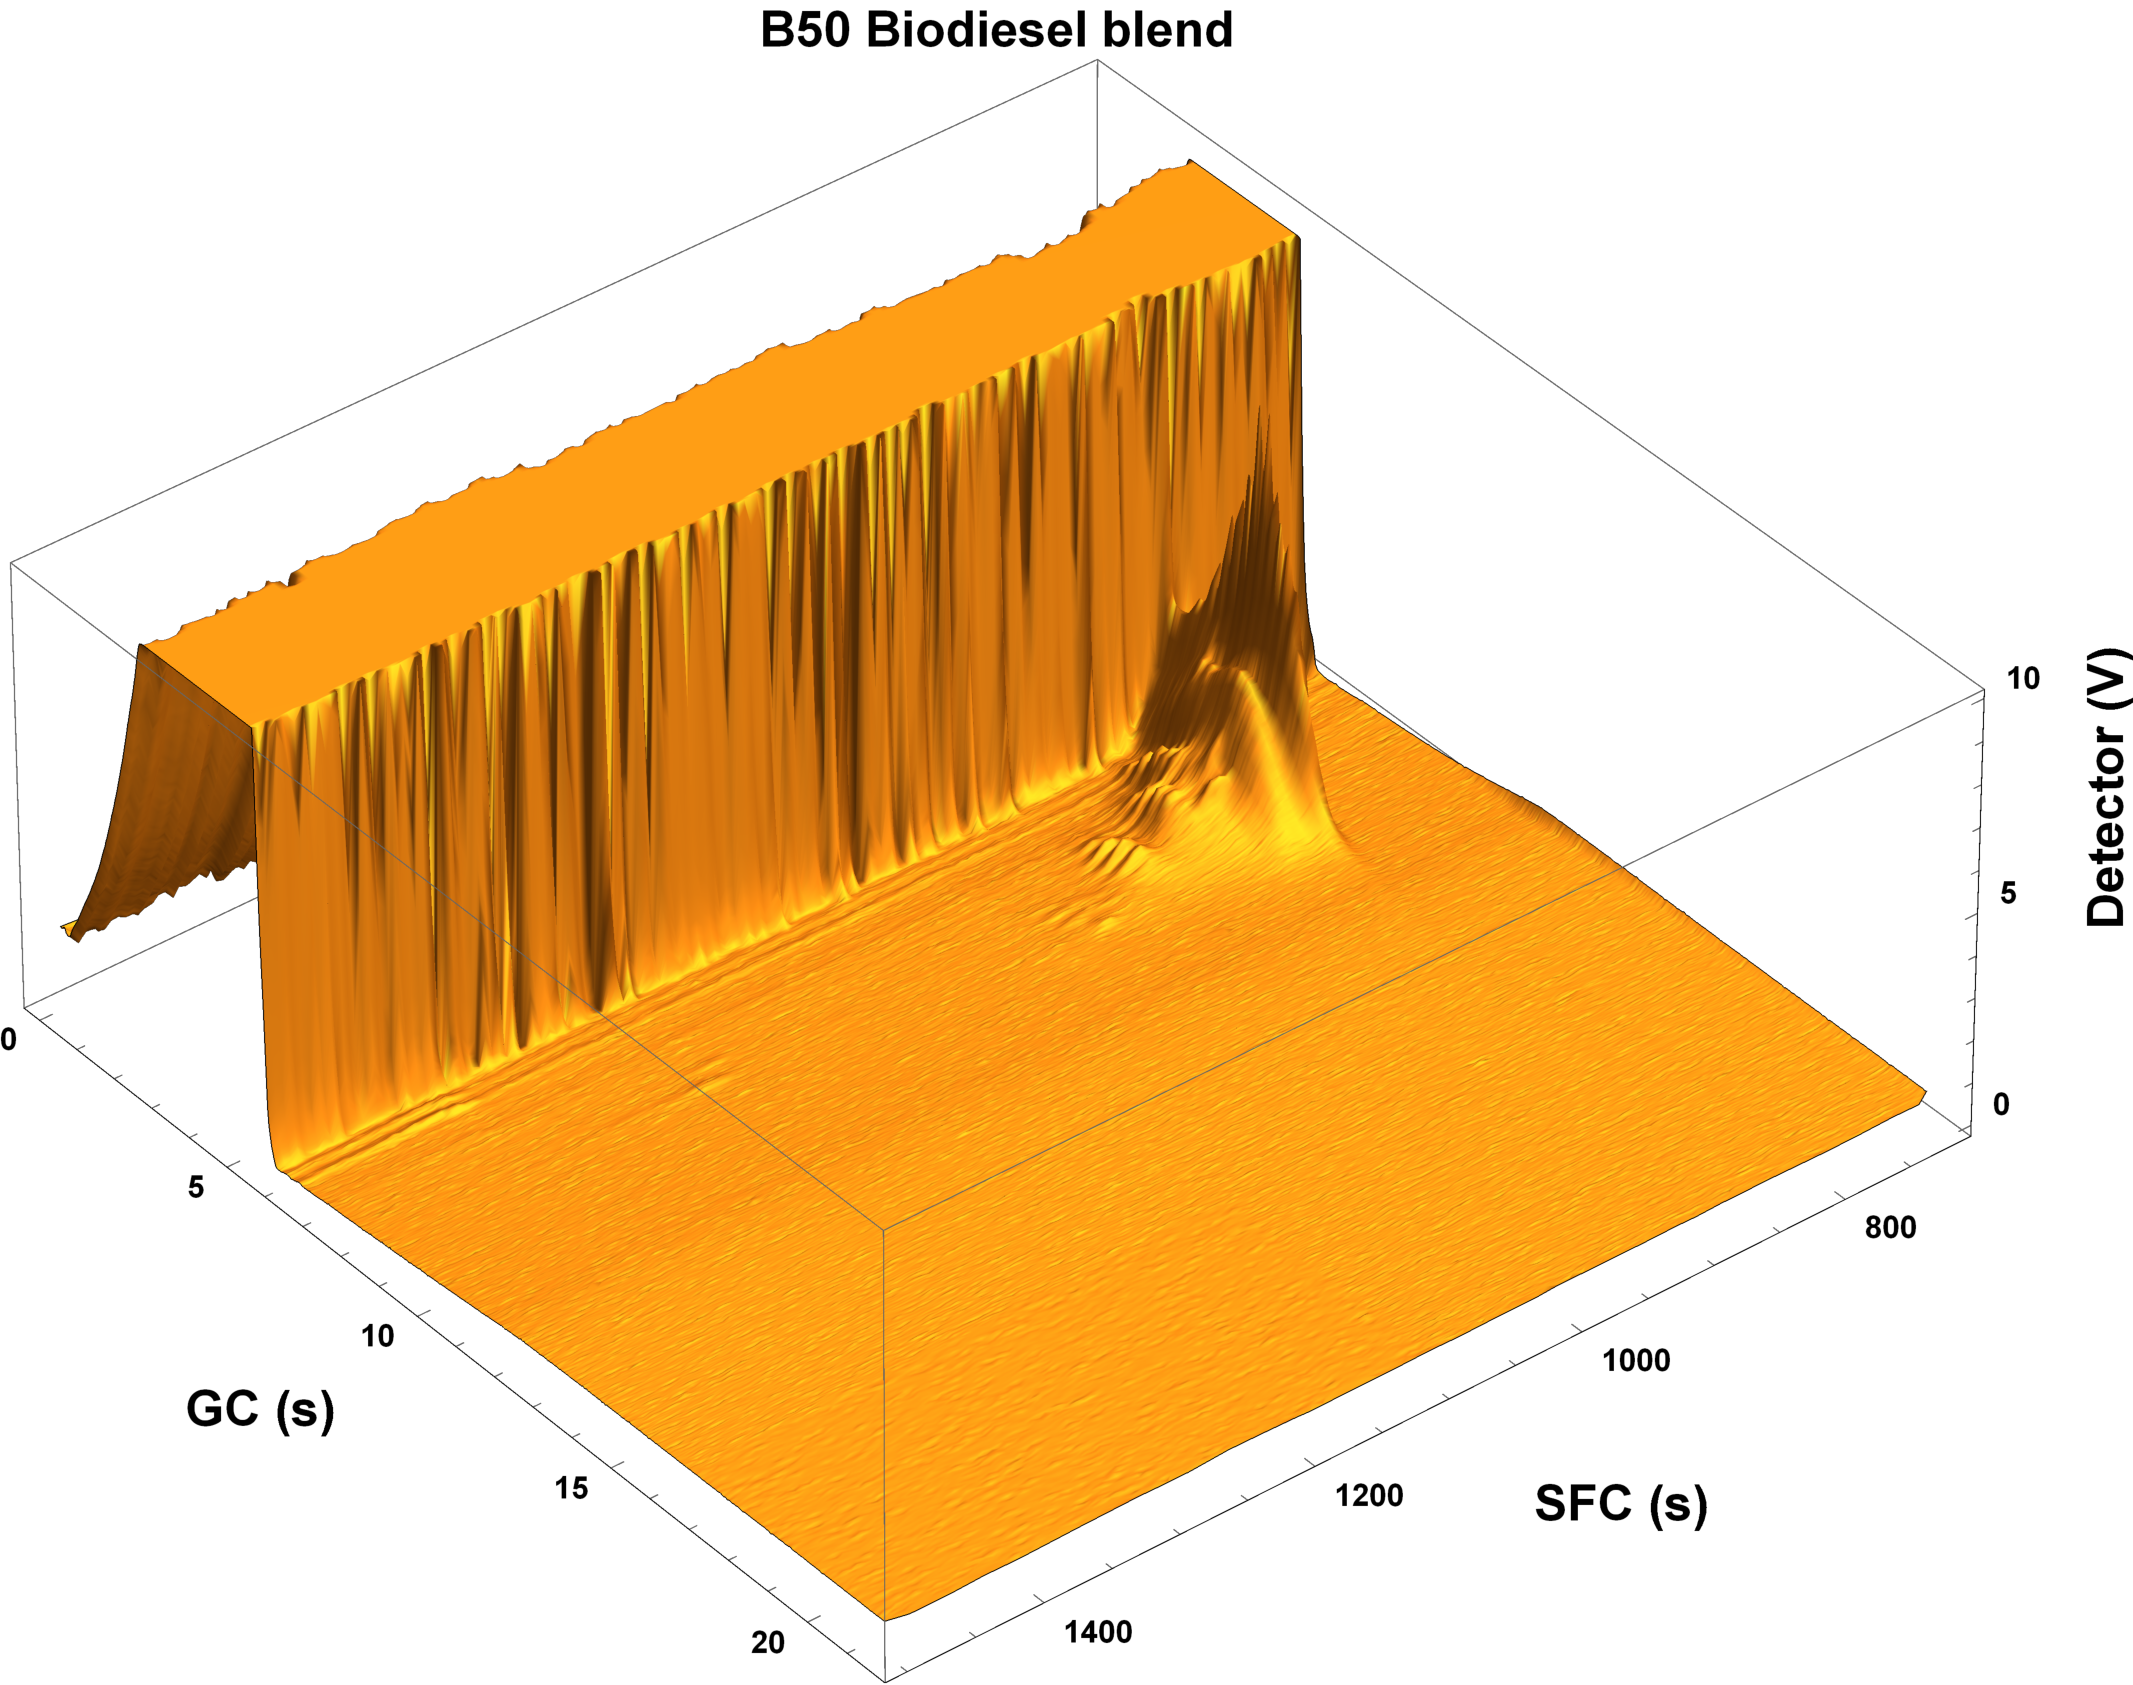
\includegraphics[width=0.8\textwidth]{Figures/Modifier.pdf}
	\decoRule	
	
	\caption[Modifiers in SFC]{The modifiers used in the SFC dimension elutes as a
solvent front on the GC dimension, and does not otherwise affect the separation.}
	
	\label{fig:Modifier} 
\end{figure}

\subsection{Discussion}